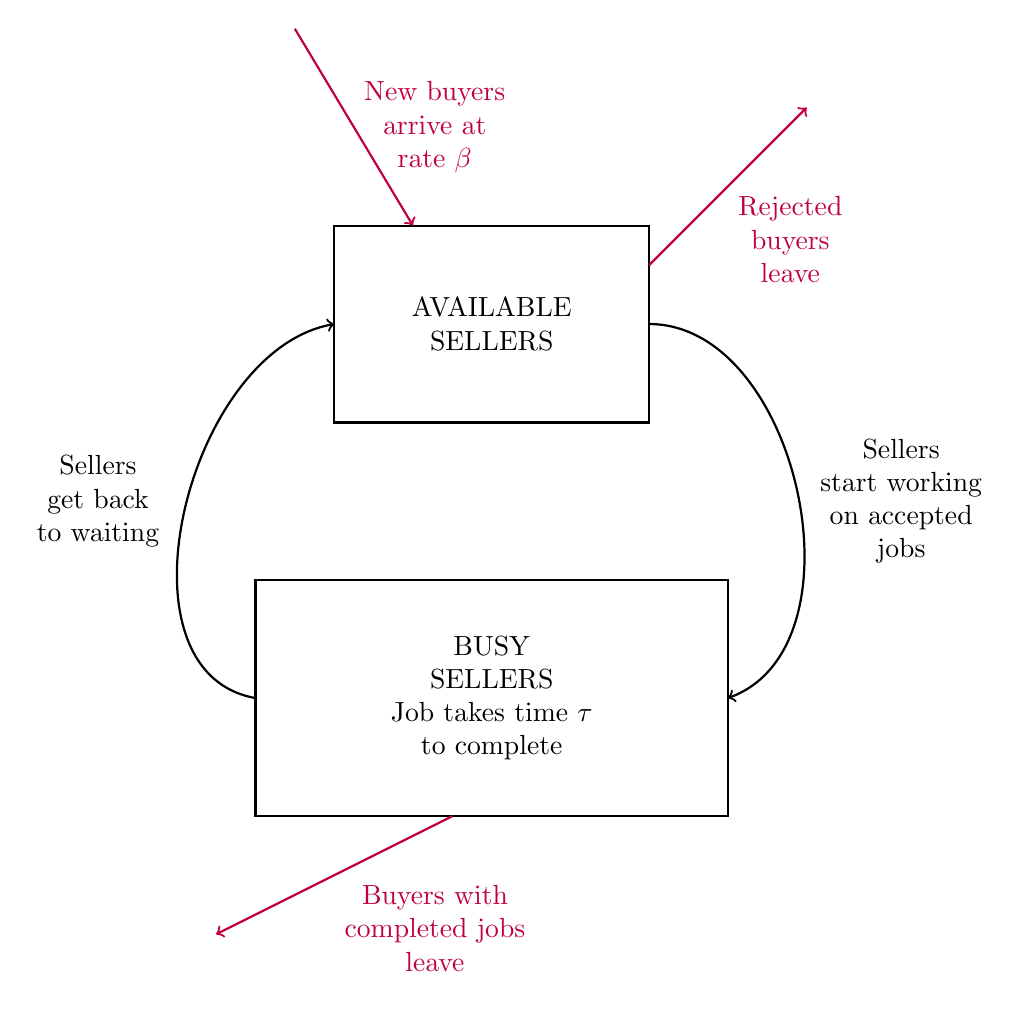
\begin{tikzpicture}[xscale=1,yscale=1,xshift=1] 


%	\draw[step=1cm,gray,very thin] (0,0) grid (10,8);

	\draw[thick] (-.5,0) rectangle (5.5,3);
	\node at (2.5,1.5) [align=center] {BUSY\\SELLERS\\ Job takes time $\tau$\\to complete};
	\draw[thick] (.5,5) rectangle (4.5,7.5);
	\node at (2.5,6.25) [align=center]  {AVAILABLE\\SELLERS};

	\draw[thick,->] (-.5,1.5) to [out=170,in=-170] (.5,6.25);
	\node at (-2.5,4) [align=center] {Sellers\\get back\\to waiting};
	\draw[thick,->] (4.5,6.25) to [out=0,in=20] (5.5,1.5);
%	\draw[thick,->,purple] (4.5,6.2) to [out=0,in=20] (5.5,1.55);
	\node at (7.7,4) [align=center] {Sellers\\start working\\on accepted\\jobs};

	\draw[thick,->,purple] (0,10) --node[align=center,right] {New buyers\\arrive at\\rate $\beta$} (1.5,7.5);
	\draw[thick,->,purple] (4.5,7) --node[align=center,below right]{Rejected\\buyers\\leave}++(2,2);
	\draw[thick,->,purple] (2,0) --node[align=center,below right]{Buyers with\\completed jobs\\leave}++(-3,-1.5);



        
\end{tikzpicture}